\documentclass[letterpaper]{article}
\usepackage[margin=1in]{geometry}
\usepackage[utf8]{inputenc}
\usepackage{textcomp}
\usepackage{amssymb}
\usepackage{natbib}
\usepackage{graphicx}
\usepackage{gensymb}
\usepackage{amsthm, amsmath, mathtools}
\usepackage[dvipsnames]{xcolor}
\usepackage{enumerate}
\usepackage{mdframed}
\usepackage[most]{tcolorbox}
\usepackage{csquotes}
% https://tex.stackexchange.com/questions/13506/how-to-continue-the-framed-text-box-on-multiple-pages

\tcbuselibrary{theorems}

\newcommand{\R}{\mathbb{R}}
\newcommand{\Z}{\mathbb{Z}}
\newcommand{\N}{\mathbb{N}}
\newcommand{\Q}{\mathbb{Q}}
\newcommand{\C}{\mathbb{C}}
\newcommand{\code}[1]{\texttt{#1}}
\newcommand{\mdiamond}{$\diamondsuit$}
\newcommand{\PowerSet}{\mathcal{P}}
\newcommand{\Mod}[1]{\ (\mathrm{mod}\ #1)}
\DeclareMathOperator{\lcm}{lcm}

%\newtheorem*{theorem}{Theorem}
%\newtheorem*{definition}{Definition}
%\newtheorem*{corollary}{Corollary}
%\newtheorem*{lemma}{Lemma}
\newtheorem*{proposition}{Proposition}


\newtcbtheorem[number within=section]{theorem}{Theorem}
{colback=green!5,colframe=green!35!black,fonttitle=\bfseries}{th}

\newtcbtheorem[number within=section]{definition}{Definition}
{colback=blue!5,colframe=blue!35!black,fonttitle=\bfseries}{def}

\newtcbtheorem[number within=section]{corollary}{Corollary}
{colback=yellow!5,colframe=yellow!35!black,fonttitle=\bfseries}{cor}

\newtcbtheorem[number within=section]{lemma}{Lemma}
{colback=red!5,colframe=red!35!black,fonttitle=\bfseries}{lem}

\newtcbtheorem[number within=section]{example}{Example}
{colback=white!5,colframe=white!35!black,fonttitle=\bfseries}{def}

\newtcbtheorem[number within=section]{note}{Important Note}{
        enhanced,
        sharp corners,
        attach boxed title to top left={
            xshift=-1mm,
            yshift=-5mm,
            yshifttext=-1mm
        },
        top=1.5em,
        colback=white,
        colframe=black,
        fonttitle=\bfseries,
        boxed title style={
            sharp corners,
            size=small,
            colback=red!75!black,
            colframe=red!75!black,
        } 
    }{impnote}
\usepackage[utf8]{inputenc}
\usepackage[english]{babel}
\usepackage{fancyhdr}
\usepackage[hidelinks]{hyperref}

\pagestyle{fancy}
\fancyhf{}
\rhead{Math 170A}
\chead{Wednesday, January 25, 2023}
\lhead{Lecture 7}
\rfoot{\thepage}

\setlength{\parindent}{0pt}

\newcommand{\0}{\mathbf{0}}
\newcommand{\y}{\mathbf{y}}
\renewcommand{\b}{\mathbf{b}}
\newcommand{\x}{\mathbf{x}}
\newcommand{\e}{\mathbf{e}}
\newcommand{\vv}{\mathbf{v}}

\begin{document}

\section{Vectors and Matrix Norms (2.1)}
In numerical analysis, we want to find approximate solutions to problems (e.g., ODEs). Some things we want to know are 
\begin{itemize}
    \item How good the approximate solution is? 
    \item How close is the approximate solution to the exact solution? 
\end{itemize}
So, \textbf{norms} are a measure of length, or the measure of being close or far apart. 

\subsection{Vector Norms}
The vector norm we're most familiar with is the one in $\R^2$, also known as the \emph{2-norm}. These might look something like
\begin{center}
    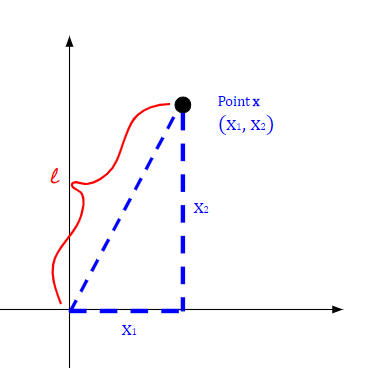
\includegraphics[scale=0.9]{../assets/v_norm.png}
\end{center}
For a point \[\x = (x_1, x_2),\] we can define the \emph{2-norm} of a vector to be \[||\x||_2 = \sqrt{x_{1}^{2} + x_{2}^{2}}.\]

\begin{definition}{Vector Norm}{}
    A \textbf{norm} of a vector (i.e., a \textbf{vector norm}) $\x \in \R^n$ is a real number $||x||$ that is assigned to $\x$. For all $\x, \y \in \R^n$ and all $c \in \R$, the following properties are satisfied: 
    \begin{enumerate}
        \item \underline{Positive Definite Property:} $||\x|| > 0$ for $\x \neq 0$ and $||\0|| = 0$. 
        \item \underline{Absolute Homogeneity:} $||c\x|| = |c| \cdot ||\x||$. 
        \item \underline{Triangle Inequality:} $||\x + \y|| \leq ||\x|| + ||\y||$. 
    \end{enumerate}
\end{definition}
\textbf{Remark:} With regards to the third property, consider \begin{center}
    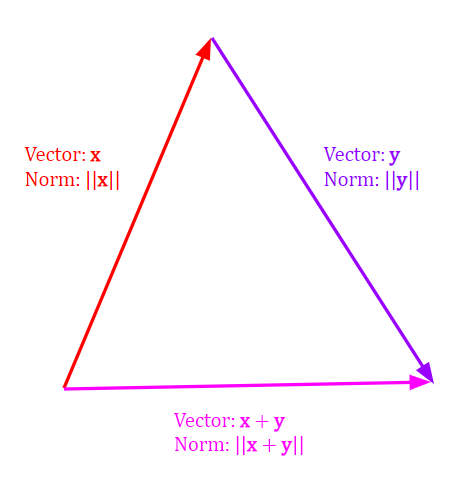
\includegraphics[scale=0.6]{../assets/tri_inequality.png}
\end{center}
Note that \[||\x + \y|| = ||\x|| + ||\y||\] if $\x$ and $\y$ points at the same direction.

\subsubsection{Popular Norms}
There are some common norms that we've seen before. As implied, they all satisfy the properties above. 
\begin{itemize}
    \item For $p \geq 1$, we define 
    \[||\x||_p = \sqrt[p]{|x_1|^p + |x_2|^p + \hdots + |x_n|^p}.\]
    Note that some special cases are 
    \[||\x||_2 = \sqrt{x_1^2 + x_2^2 + \hdots + x_n^2}\]
    and 
    \[||\x||_1 = |x_1| + |x_2| + \hdots + |x_n| = \sum_{i = 1}^{n} |x_i|.\]

    \item The infinite norm is defined to be \[||\x||_{\infty} = \max_{i = 1, 2, \hdots, n} |x_i|.\] It should be noted that \[\lim_{p \mapsto \infty} ||\x||_p = ||\x||_{\infty}.\]
\end{itemize}

\subsection{Matrix Norms}
We now want to consider norms for a matrix $A \in \R^{n \times n}$. There are two ways we can interpret matrix norms.
\begin{enumerate}
    \item Interpret matrix as a vector. For example, suppose we have \[A = \begin{bmatrix}
        -1 & 0 & 5 \\ 8 & 2 & 7 \\ -3 & 1 & 0
    \end{bmatrix}.\] Then, we can ``convert'' this matrix to a vector like so: \[\vv = \begin{bmatrix}
        -1 \\ 0 \\ 5 \\ 8 \\ 2 \\ 7 \\ -3 \\ 1 \\ 0
    \end{bmatrix}.\] Here, $\vv \in \R^9$. Notice how the first column of $A$ is the top three elements in $\vv$, the second column of $A$ is the middle three elements of $\vv$, and the last column of $A$ is the bottom three elements of $\vv$. 

    \item We can also define the matrix as a linear operator. That is, for a function $L: \R^n \mapsto \R^n$, we have \[L(\x) = A\x.\]
\end{enumerate}

\subsubsection{General Definition of Matrix Norms}
\begin{definition}{Matrix Norm}{}
    A \textbf{matrix norm} assigns a real number $||A||$ to a matrix $A$. This should satisfy the following conditions for all $A, B \in \R^{n \times n}$ and $c \in \R$. 
    \begin{enumerate}
        \item $||A|| > 0$ if $A \neq 0$, and $||0|| = 0$. 
        \item $||cA|| = |c| \cdot ||A||$. 
        \item $||A + B|| \leq ||A|| + ||B||$.
        \item Submultiplicity: $||AB|| \leq ||A|| \cdot ||B||$.  
    \end{enumerate}
\end{definition}
\textbf{Remark:} Regarding submultiplicity, for any $\x, \y \in \R^n$, we have \[|\cyclic{x, y}| \leq ||\x||_2 ||y||_2,\] known as the Cauchy Schwarz inequality. 

\subsubsection{Vector Viewpoint}
Going back to the vector viewpoint, let's suppose we have \[A = \begin{bmatrix}
    a_{11} & a_{12} & \hdots & a_{1n} \\ 
    a_{21} & a_{22} & \hdots & a_{2n} \\ 
    \vdots & \vdots & \ddots & \vdots \\ 
    a_{n1} & a_{n2} & \hdots & a_{nn}
\end{bmatrix}.\] Then, 
\[\vv = \begin{bmatrix}
    a_{11} \\ a_{21} \\ \vdots \\ a_{n1} \\ a_{12} \\ a_{22} \\ \vdots \\ a_{n2} \\ \vdots \\ a_{1n} \\ a_{2n} \\ \vdots \\ a_{nn}
\end{bmatrix}.\]

The Frobenius norm of $A$ is defined by 
\[||A||_F = ||\vv||_2 = \left(\sum_{i = 1}^{n} \sum_{j = 1}^{n} |a_{ij}|^2\right)^{\frac{1}{2}}.\]

\subsubsection{Matrix Norm}
Matrix $p$-norms are defined as follows: 
\[||A||_p = \max_{\substack{\x \in \R^n \\ \x \neq \0}} \frac{||A\x||_p}{||\x||_p}.\]
This measures the \emph{maximum stretch} the linear function $L(\x) = A\x$ can do to a vector (normalized by the length of the vector).

\bigskip 

Some of the most important matrix $p$-norms are 
\begin{itemize}
    \item For $p = 1$: $||A||_1 = \max_{\x \neq \0} \frac{||A\x||_1}{||\x||_1} = \max_{j = 1, 2, \hdots, n} \sum_{i = 1}^{n} |a_{ij}|.$ (maximum $L_1$-norm of each column.) 
    \item For $p = \infty$: $||A||_\infty = \max_{\x \neq \0} \frac{||A\x||_\infty}{||\x||_\infty} = \max_{i = 1, 2, \hdots, n} \sum_{j = 1}^{n} |a_{ij}|.$ (maximum $L_1$-norm of each row.)
    \item For $p = 2$: $||A||_2 = \max_{\x \neq \0} \frac{||A\x||_2}{||\x||_2} = \sigma_1.$ (largest\footnote{This is related to SVD, which we will learn later.} singular value of matrix $A$.)
\end{itemize}
\textbf{Remark:} Don't confuse $||A||_2$ and $||A||_F$. They are very different! Specifically, 
\[||A||_2 = \max_{\x \neq \0} \frac{||A\x||_2}{||\x||_2}\]
while 
\[||A||_F = ||\vv||_2 = \left(\sum_{i, j} (a_{ij})^2\right)^{\frac{1}{2}}.\]

\end{document}